% Created 2022-07-27 水 15:45
% Intended LaTeX compiler: pdflatex
\documentclass[11pt]{scrartcl}
                 \usepackage[utf8]{inputenc}
                 \usepackage{cmbright}
                 \usepackage[usenames,dvipsnames]{xcolor}
                 \usepackage{graphicx,longtable,url,rotating}
                 \usepackage{amsmath}
                 \usepackage{amsfonts}
                 \usepackage{amssymb}
                 \usepackage{subfig}
                 \usepackage{minted}
                 \usepackage{algpseudocode}
                 \usepackage[round]{natbib}
                 \usepackage{alltt}
                 \renewenvironment{verbatim}{\begin{alltt} \scriptsize \color{Bittersweet} \vspace{0.2cm} }{\vspace{0.2cm} \end{alltt} \normalsize \color{black}}
\definecolor{lightcolor}{gray}{.55}
\definecolor{shadecolor}{gray}{.95}
\usepackage{multicol}

                 \usepackage{hyperref}
                 \hypersetup{colorlinks=true,pagebackref=true,urlcolor=orange}
\author{Nilton Liuji Kamiji, Christophe Pouzat, Aline Duarte, Antonio Roque, \\Antonio Galves}
\date{\today}
\title{Implementaion of the Potjans Diesmann microcircuit model using the classical Galves-L\"{o}cherbach neuron model}
\hypersetup{
 pdfauthor={Nilton Liuji Kamiji, Christophe Pouzat, Aline Duarte, Antonio Roque, \\Antonio Galves},
 pdftitle={Implementaion of the Potjans Diesmann microcircuit model using the classical Galves-L\"{o}cherbach neuron model},
 pdfkeywords={},
 pdfsubject={},
 pdfcreator={Emacs 27.2 (Org mode 9.4.4)}, 
 pdflang={English}}
\begin{document}

\maketitle
\tableofcontents
\pagebreak
\listoffigures
\pagebreak

\section{Model considered}
\label{sec:org8d5c27a}
\subsection{The original PD model}
\label{sec:orga57681e}
\label{org436adc3}

The PD model (Potjans and Diesmann, 2014) consists of 8 neuronal populations, representing excitatory and inhibitory populations of 4 cortical layers, namely, layers 2/3 (L23e/i), 4 (L4e/i), 5 (L5e/i) and 6 (L6e/i), where e denotes excitatory and i inhibitory. The number of neurons of each population is shown in table \ref{table:PD_num_neurons}, which totalizes 77169 neurons.
\begin{table}[htbp]
    \centering
    \caption{Number of neurons per cortical layer}
    \label{table:PD_num_neurons}
    \begin{tabular}{llllllll}
         \multicolumn{1}{c}{L23e} & \multicolumn{1}{c}{L23i} & \multicolumn{1}{c}{L4e} & \multicolumn{1}{c}{L4i} & \multicolumn{1}{c}{L5e} & \multicolumn{1}{c}{L5i} & \multicolumn{1}{c}{L6e} & \multicolumn{1}{c}{L6i} \\
         20683 & 5834 & 21915 & 5479 & 4850 & 1065 & 14395 & 2948 
    \end{tabular}
\end{table}

\subsubsection{Membrane potential dynamics}
\label{sec:org9141b64}
\label{org15d6235}

All neurons are described with the same LIF (leaky integrate-and-fire) dynamics (eq. (\ref{eq:LIF}))
\begin{equation}
  \begin{aligned}
    \frac{dV_m(t)}{dt} &= \begin{cases} 0 & \text{if neuron is refractory} \\
    -\frac{V_m(t)}{\tau_m} + \frac{S_{syn}^i(t)}{C_m} & \text{otherwise}
    \end{cases} \\
    \frac{dI_{syn}(t)}{dt} &= \begin{cases} 0 & \text{if neuron is refractory} \\
    -\frac{I_{syn}(t)}{\tau_{syn}} + \sum_j{W_j} & \text{otherwise}
    \end{cases} \\
    \text{if } V_m^i(t) \geq V_{th} &\quad \text{neuron spiked and refractory}
  \end{aligned}
  \label{eq:LIF}
\end{equation}
where \(V_m(t)\) is the membrane potential, \(\tau_m = 10\) ms is the membrane time constant representing the leakage effect, \(C_m = 250\) pF the membrane capacitance, \(V_{th} = 15\) mV the threshold potential in which a neuron fires when its membrane potential exceeds this value, \(I_{syn}(t)\) the membrane current elicited by synaptic inputs from pre-synaptic neurons  \(j\) (\(W_j\)), and \(\tau_{syn} = 0.5\) ms the synaptic time constant indicating the dynamics of synaptic receptor channel. The refractory period (\(\tau_{ref}\)), the period in which a neuron stays silent after emmiting a spike, was 2 ms.


\subsubsection{The graph of interaction}
\label{sec:org0b83022}
\label{orgcf3250b}

Neurons are connected following the connection probability between neuronal populations shown in table \ref{table:PD_conectivity}.
The resulting graph of interaction is a directed graph with nearly 300 million edges.

\begin{table}[htbp]
    \centering
    \caption{\label{table:PD_conectivity} Connection probability between neuronal populations
    }
    \begin{tabular}{lccccccccc}
         &  & \multicolumn{8}{c}{from} \tabularnewline
         &  & L23e & L23i & L4e & L4i & L5e & L5i & L6e & L6i \tabularnewline
         & L23e & 0.101 & 0.169 & 0.044 & 0.082 & 0.032 & 0.0 & 0.008 & 0.0 \tabularnewline
         & L23i & 0.135 & 0.137 & 0.032 & 0.052 & 0.075 & 0.0 & 0.004 & 0.0 \tabularnewline
         & L4e & 0.008 & 0.006 & 0.050 & 0.135 & 0.007 & 0.0003 & 0.045 & 0.0 \tabularnewline
         to & L4i & 0.069 & 0.003 & 0.079 & 0.160 & 0.003 & 0.0 & 0.106 & 0.0 \tabularnewline
         & L5e & 0.100 & 0.062 & 0.051 & 0.006 & 0.083 & 0.373 & 0.020 & 0.0 \tabularnewline
         & L5i & 0.055 & 0.027 & 0.026 & 0.002 & 0.060 & 0.316 & 0.009 & 0.0 \tabularnewline
         & L6e & 0.016 & 0.007 & 0.021 & 0.017 & 0.057 & 0.020 & 0.040 & 0.225 \tabularnewline
         & L6i & 0.036 & 0.001 & 0.003 & 0.001 & 0.028 & 0.008 & 0.066 & 0.144 
         \tabularnewline
    \end{tabular}
\end{table}

Moreover, synaptic connections between neurons \(j\) and \(i\) are described by the synaptic weights (\(w_{j \to i}\)) and transmission delay (\(d_{j \to i}\)), drawn from a clipped normal distribution, and are different for excitatory and inhibitory synapses as shown in table \ref{table:PD_synaptic_weight_delay}. \(dt\) is the simulation time step, indicating that synapse transmission requires at least one time step.

\begin{table}[htb!]
    \centering
    \caption{Synaptic weight and delay. Synaptic weights are clipped at 0, and synaptic delays are clipped at simulation step ($d_t = 0.1$ ms)}
    \label{table:PD_synaptic_weight_delay}
    \begin{tabular}{lcl}
        %  \multicolumn{2}{c}{excitatory} \\
         &
         $w_e$ & $\mathcal{N}$($\mu = 87.8, \sigma = 8.8$) pA; $w_e > 0$ \\
         excitatory & $d_e$ & $\mathcal{N}$($\mu=1.5 , \sigma = 0.75$) ms; $d_e \geq dt$ \\
        %  \multicolumn{2}{c}{inhibitory}  \\
         &
         $w_i$ & $\mathcal{N}$($\mu = -351.2, \sigma = 35.1$) pA; $w_i < 0$ \\
         inhibitory & $d_i$ & $\mathcal{N}$($\mu=0.8 , \sigma = 0.4$) ms; $d_i \geq dt$
    \end{tabular}
\end{table}

\textbf{Remark 1} A synaptic weight of \(87.8\) pA will elicit a maximum membrane potential change of approximately \(0.15\) mV.

\textbf{Remark 2} The number of synapses (\(K\)) between any two populations are calculated from:
\begin{equation}
    K = \frac{\log(1 - C_a)}{\log(1-1/(N_{pre}N_{post}))},
    \label{eq:PD_K}
\end{equation}
where \(C_a\) is the connection probability taken from table \ref{table:PD_conectivity}, \(N_{pre}\) and \(N_{post}\) the number of neurons in the pre- and post-synaptic population, respectively, taken from table \ref{table:PD_num_neurons}. The \(K\) pairs are then randomly chosen, so that multiple synapses with different parameter values for any pair can occur. This phenomenon is know as multapses.

\textbf{Remark 3} The connection weight between neurons of L4e to L23e is doubled, that is, taken from a clipped normal distribution of \(\mathcal{N}\)(\(\mu = 175.6, \sigma = 17.6\)) pA

\subsubsection{Background input}
\label{sec:orgdf688cb}
\label{org4820a61}

The network is driven by a constant external input that can be described as Poissonian spike trains (\(rate = 8\) Hz) or constant current. The number of external inputs is layer dependent as shown in table \ref{table:PD_ext_num_neurons}.

\begin{table}[htbp]
    \centering
    \caption{Number of external inputs onto each cortical layer}
    \label{table:PD_ext_num_neurons}
    \begin{tabular}{llllllll}
         \multicolumn{1}{c}{L23e} & \multicolumn{1}{c}{L23i} & \multicolumn{1}{c}{L4e} & \multicolumn{1}{c}{L4i} & \multicolumn{1}{c}{L5e} & \multicolumn{1}{c}{L5i} & \multicolumn{1}{c}{L6e} & \multicolumn{1}{c}{L6i} \\
         1600 & 1500 & 2100 & 1900 & 2000 & 1900 & 2900 & 2100 
    \end{tabular}
\end{table}

\textbf{Remark 1} In the case of Poissonian spike trains input, every neuron on each layer receives independent Poissonian spike trains with \(rate = 8 \times n\), where \(n\) is the number of external inputs, which is the same as generating \(n\) Poissonian spike trains of \(8\) Hz and applying all of it to the neuron. Note that all input has fixed weight and delay values of \(87.8\) pA and \(1.5\) ms, respectively.

\subsection{The GL model}
\label{sec:org2652c4d}
\label{org98b0484}

We consider a network made of (N) neurons in a discrete time setting. We write \(I = \{1,\ldots,N\}\) the neurons' index set. The neurons can be viewed as the nodes of a \emph{directed graph}. The synapses between neurons / edges of the graph are specified by a quadruple:
\begin{description}
\item[{\(j \in I\)}] The \emph{.presynaptic neuron}.
\item[{\(i \in I\)}] The \emph{postsynaptic neuron}.
\item[{\(w_{j\rightarrow i} \in \mathbb{R}\)}] The \emph{synaptic weight}, if \(w_{j\rightarrow i} = 0\) there is no synapse from \(j\) to \(i\), if \(w_{j\rightarrow i} < 0\) the synapse is \emph{inhibitory}, if \(w_{j\rightarrow i} >0\) it is \emph{exitatory}.
\item[{\(d_{j\rightarrow i} \in \mathbb{R}^+\)}] The \emph{synaptic delay}, this accounts for the \emph{propagation time} of the spike from the soma of neuron \(j\) to the the synaptic terminal on neuron \(i\), as well as the time for the presynaptic vesicles to fuse upon spike arrival, the transmitter to diffuse and bind to the postsynaptic receptors and the latter to open.
\end{description}

\subsection{Spike trains}
\label{sec:org976a227}
A \emph{spike train} is associated with each neuron, \(i\), of the network. This is a sequence of random variables \(X_t(i)\), where \(t\) is the discrete time index, taking value in \(\{0,1\}\). \(X_t(i) = 0\) means that neuron \(i\) does not spike at time \(t\), while \(X_t(i) = 1\) means neuron \(i\) spikes at time \(t\). 

\textbf{Last spike time} We are going to consider models with membrane potential reset (see next section) following a spike. This will force us to refer to the \emph{last spike time of neuron \(i\) before time \(t\)}, \(L_t (i)\):
\begin{equation}\label{eq:last-spike-time}
L_t (i) = \max \{ s \le  t  : X_s (i) = 1  \} \,.
\end{equation}  

\subsection{Membrane potential and rate function}
\label{sec:orgbddb1e4}

With every neuron \(i\) we associate a \emph{Membrane Potential Process} \(V_t(i)\) and a \emph{rate function} \(\phi_i: \mathrm{R} \mapsto [0,1]\). Given the \(\{V_t(i)\}_{i \in I}\), each neuron spikes at time \(t+1\) \textbf{independently of the others} with probability \(\phi_i\left(V_t(i)\right)\). 

\emph{In the absence of input} the membrane potential of each neuron decays spontaneously and \emph{deterministically} according to:
\begin{equation}\label{eq:leakage}
V_{t+1}(i) = \rho V_{t}(i), \quad 0 < \rho \le 1\, , 
\end{equation}  
this dynamics reflects the membrane potential leakage. \(\rho\) could clearly be made neuron specific or specific to a neuron class (exitatory / inhibitory neurons for instance).

\subsection{Synaptic input}
\label{sec:orgb302461}

If \(w_{j\rightarrow i} \neq 0\), a spike in neuron \(j\) will influence the membrane potential of neuron \(i\) (and its subsequent probability of spiking) with a delay \(d_{j\rightarrow i}\). Since we are considering a model with "comprehensive reset following a spike" only the spikes \emph{arriving} after the last spike of neuron \(i\), (\(L_t (i)\)) are going to contribute. We must therefore only consider a subset of the time indices, namely: $$\{s: X_s(j)+d_{j\rightarrow i} > L_t (i)\}\,.$$
A last feature of synapses that we might want to consider is the fact that synaptic conductances remain open (or active) for a finite amount of time and decay (roughly) mono-exponentially. We will therefore model the effect of a spike in neuron \(j\) at time \(X_s(j)\) on the membrane potential of neuron \(i\) by:
\begin{equation}\label{eq:single-input-effect}
w_{j\rightarrow i} \xi^{t-s-d_{j\rightarrow i}} X_s(j), \; X_s(j)+d_{j\rightarrow i} > L_t (i) \text{ and } 0 \le \xi \le 1\, ,
\end{equation}
where \(\xi\) accounts for the synaptic conductance dynamics. If it is null since \(0^0=1\) the synaptic input is limited to the time at which the presynaptic spike arrives. Again parameter \(\xi\) could be made synapse or synapse type (exitatory \emph{vs} inhibitory) specific.

The last assumption we need is the \textbf{linear summation} on the membrane potential of all the synaptic inputs received by a given neuron in the absence of spike of the latter.

\subsection{Overall dynamics}
\label{sec:org6195c6e}
In practice a sequence of Bernoulli random variable is used at each time step: \(\{U_t(i)\}_{i \in I}\), \(U_t(i) \stackrel{IID}{\sim} \mathcal{B}\) and the \(V_{t+1}(i)\) are given by:
\begin{equation}\label{eq:V-evolution}
V_{t+1}(i) = \begin{cases}0 & \text{if } U_t(i) \le \phi_i\left(V_t(i)\right) \\ \rho V_{t}(i) + \sum_{j \in I}  w_{ j \to i} \left( \sum_{ s = L_t (i) +1 -d_{j\rightarrow i} }^{ t-d_{j\rightarrow i}}\xi^{t-s-d_{j\rightarrow i}}X_s (j)  \right) & \text{otherwise}   \end{cases}
\end{equation} 
and
\begin{equation}\label{eq:X-evolution}
X_{t+1}(i) = \begin{cases}1 & \text{if } U_t(i) \le \phi_i\left(V_t(i)\right) \\ 0 & \text{otherwise}   \end{cases}
\end{equation}

\textbf{Remark 1} If \(\xi=0\) and \(d_{j\rightarrow i} = 0\) for all \((i,j) \in I^2\), then Eq. \ref{eq:V-evolution} becomes much simpler, namely:
\begin{equation}\label{eq:V-evolution-simple}
V_{t+1}(i) = \begin{cases}0 & \text{if } U_t(i) \le \phi_i\left(V_t(i)\right) \\ \rho V_{t}(i) + \sum_{j \in I}  w_{ j \to i} X_t (j)  & \text{otherwise}   \end{cases}
\end{equation} 
and we see that the knowledge of the \(\{V_t(i)\}_{i \in I}\),  the \(\{X_t(i)\}_{i \in I}\) and the \(\{U_t(i)\}_{i \in I}\) is enough to get both the \(\{V_{t+1}(i)\}_{i \in I}\) and the \(\{X_{t+1}(i)\}_{i \in I}\), a nice Markovian setting.

\textbf{Remark 2} If \(\xi=0\) and \(d_{j\rightarrow i} \le d_{max}\) for all \((i,j) \in I^2\) then Eq. \ref{eq:V-evolution} is still "simple" but not as simple as Eq. \ref{eq:V-evolution-simple}, namely:
\begin{equation}\label{eq:V-evolution-not-so-simple}
V_{t+1}(i) = \begin{cases}0 & \text{if } U_t(i) \le \phi_i\left(V_t(i)\right) \\ \rho V_{t}(i) + \sum_{j \in I}  w_{ j \to i} X_{t-d_{j\rightarrow i}}(j) & \text{otherwise}   \end{cases}
\end{equation} 
and the the knowledge of the \(\{V_t(i)\}_{i \in I}\), the \(\{X_t(i)\}_{(t,i) \in \{t-d_{max},\ldots,t\} \times I}\) and the \(\{U_t(i)\}_{i \in I}\) is enough to get both the \(\{V_{t+1}(i)\}_{i \in I}\) and the \(\{X_{t+1}(i)\}_{i \in I}\), a not so nice but still  Markovian setting.

\color{gray}
\textbf{Remark 3} In the general case where \(\xi > 0\), the Markovian setting is lost since we might need to go back an infinite number of time steps in the past in order to compute \(V_{t+1}(i)\). 

\textbf{Remark 4}
\color{red}
In equation (\ref{eq:V-evolution}), one has to always go back to \(L_t(i)\) on every evaluation of \(V_t(i)\). This would be computationally inefficient. If we add an auxiliary variable to track only the synaptic inputs (lets call it \(S_t^{syn}(i)\)), eq. (\ref{eq:V-evolution}) can be extended to the following set of equations:

\color{black}
\begin{equation}\label{eq:V-evolution-extended}
V_{t+1}(i) = \begin{cases}0 & \text{if } U_t(i) \le \phi_i\left(V_t(i)\right) \\
% 0 & \text{if } L_t(i) \le t \le L_t(i) + \tau_{ref} \\
\rho V_{t}(i) + \zeta \left(S_t^{syn}(i) + S_t^{ext}(i)\right) & \text{otherwise}   \end{cases}
\end{equation} 
and

\begin{equation}\label{eq:Isyn-evolution-refractory}
S_{t+1}^{syn}(i) = \begin{cases}
% 0 & \text{if } L_t(i) \le t \le L_t(i) + \tau_{ref} \\
0 & \text{if } U_t(i) \le \phi_i\left(V_t(i)\right) \\
\xi S_t^{syn}(i) + \sum_{j \in I}  w_{ j \to i} X_{t{\color{red}+1}-d_{j\rightarrow i}}(j) & \text{otherwise}   \end{cases}
\end{equation} 
where \(\zeta\) is a conversion factor from synaptic current to membrane potential.

\color{red}
\textbf{Remark 5} I'm still thinking how delay should be correctly implemented in eq. (\ref{eq:Isyn-evolution-refractory}). Although it was discussed that \(X_{t-d_{j \to i}}(j)\) should be used, discretization method introduced in Rotter and Diesmann (1999) suggests the use of \(X_{t+1-d_{j \to i}}(j)\). The difference should be negligible, but which one is more likely to be correct?

\textbf{Remark 6} How to correctly implement refractory period (\(\tau_{ref}\)), the time during which  neuron remains silent after emmiting a spike? To a first approximation I will implement following the method applied in the PD model, but they just keep the membrane potential at zero, but do not reset synaptic current. The discussion on the meeting was that synaptic current should also be reset!

\color{black}

\textbf{Remark 7} \(\tau_{ref}\) was not considered in eqs. (\ref{eq:V-evolution} -- \ref{eq:V-evolution-not-so-simple}), as this was not discussed on the previous meeting.

\section{Codes}
\label{sec:org8c29d2c}
The coming examples assume that \texttt{Python 3} is used.

\subsection{Spike trains representation}
\label{sec:org781067f}

\subsubsection{Binary sequences as unsigned integers}
\label{sec:org5b9dd0f}
A spike train \emph{realization} is a sequence of 0 and 1 like: \texttt{00100101000010001}. It can also be viewed as a non-negative (unsigned) integer, assuming that \(K\) time steps are considered, \(\{x_{i}=0,x_{i+1}=0,x_{i+2}=1,\ldots,x_{i+K}=1\}\) can be mapped to the integer: $$S=x_{i} 2^{K-1}+x_{i+1} 2^{K-2} + \cdots + x_{i+K} 2^0\,.$$ A nice feature of integer representation in \texttt{Python} is that: \href{https://docs.python.org/3/library/stdtypes.html\\\#typesnumeric}{Integers have unlimited precision}; stated differently integers are memory (RAM size) limited. This is a very specific feature of \texttt{Python}, most languages impose a limit (upper bound) to (unsigned) integers, typically \(2^{32}-1\)
 of \(2^{64}-1\). A binary sequence like the one we just wrote, \texttt{00100101000010001}, can be directly converted into a integer with:

\begin{minted}[bgcolor=shadecolor,fontsize=\scriptsize]{python}
int(0b00100101000010001)
\end{minted}

\begin{verbatim}
18961
\end{verbatim}



Notice the \texttt{0b} prefix, that's the way to declare a binary literal in \texttt{Python}, see the \href{https://docs.python.org/3/library/functions.html?highlight=bin\\\#int}{int} function documentation. Function \href{https://docs.python.org/3/library/functions.html?highlight=bin\\\#bin}{bin} allows us to go the other way around:

\begin{minted}[bgcolor=shadecolor,fontsize=\scriptsize]{python}
bin(18961)
\end{minted}

\begin{verbatim}
'0b100101000010001'
\end{verbatim}



Notice here that the sequence starts (necessarily) with a \texttt{1} on the left (after the \texttt{0b} prefix). This implies that if we want to represent our spike train realizations with (unsigned) integers we must keep track of our sequence lengths in order to add extra \texttt{0} on the left side if necessary..  

\subsubsection{Adding an event (spike or no spike) to a sequence}
\label{sec:orgbca973b}

Adding a "no spike" event to a sequence is trivial we just multiply it by 2 or we \href{https://docs.python.org/3/library/stdtypes.html\\\#bitwise-operations-on-integer-types}{shift it} one \texttt{bit} to the left:

\begin{minted}[bgcolor=shadecolor,fontsize=\scriptsize]{python}
bin(18961 << 1)
\end{minted}

\begin{verbatim}
'0b1001010000100010'
\end{verbatim}


To add a "spike" event we shift one \texttt{bit} to the left and add 1:

\begin{minted}[bgcolor=shadecolor,fontsize=\scriptsize]{python}
bin((18961 << 1)+1)
\end{minted}

\begin{verbatim}
'0b1001010000100011'
\end{verbatim}

\subsubsection{Finding if there was a spike 5 steps ago}
\label{sec:org4f7ee0a}
If we want to know if there was a spike 5 steps ago, we make a right shift of 5 \texttt{bit} before making a bitwise \texttt{and} with \texttt{1}:

\begin{minted}[bgcolor=shadecolor,fontsize=\scriptsize]{python}
(18961 >> 5) & 1
\end{minted}

\begin{verbatim}
0
\end{verbatim}



If we try 9 steps ago we get:

\begin{minted}[bgcolor=shadecolor,fontsize=\scriptsize]{python}
(18961 >> 9) & 1
\end{minted}

\begin{verbatim}
1
\end{verbatim}


\subsection{Simulating membrane dynamics with synaptic input (PD model case)}
\label{sec:org1cd5277}

\subsubsection{Simulating the stochastic PD model: discrete version}
\label{sec:org4787dcf}

We first consider a discrete simulation with time step of 0.1 ms (\(d_t = 0.1\) ms), which is the same of the original PD model simulated in NEST.

Under this condition (\(d_t=0.1\) ms) and considering the following parameter values: \(\tau_m = 10\) ms, \(C_m = 250\) pF, \(\tau_{syn} = 0.5\) ms, the set of equation to simulate is:
\begin{align}\label{eq:discrete-PD}
V_{t+1}(i) = \begin{cases}0 & \text{if } U_t(i) \le \phi_i\left(V_t(i)\right) \\
\rho V_{t}(i) + S_t^{syn}(i) + S_t^{ext} & \text{otherwise}   \end{cases} \\
S_{t+1}^{syn}(i) = \begin{cases}0 & \text{if } L_t(i) \le \tau_{ref} \\
\xi S_t^{syn}(i) + \sum_{j \in I_{exc}} \zeta w_{ j \to i} X_{t-d_{j\rightarrow i}}(j) - \sum_{j \in I_{inh}} g \zeta w_{ j \to i} X_{t-d_{j\rightarrow i}}(j) & \text{otherwise}   \end{cases}
\end{align}
where \(I_{exc}\) is the set of excitatory neurons, \(I_{inh}\) the set of inhibitory neurons, \(g=4\) (the ratio between inhibitory and excitatory synaptic weight), \(\rho=e^{-d_t/\tau_m}\approx0.99\), \(\xi=e^{-d_t/\tau_{syn}}\approx0.82\), \(\zeta=\left(e^{-d_t/\tau_m}-e^{-d_t/\tau_{syn}}\right)/\left(1/\tau_{syn}-1/\tau_m\right)C_m\approx0.00036\) ms/pF and \(\tau_{ref}=2.0\) ms. Moreover, \(w_{j\to i}=\mathcal{N}\left(\mu=87.8, \sigma=8.8\right)\) pA and \(d_{j\to i}=\mathcal{N}\left(\mu=1.5, \sigma=0.75\right)\) ms, and \(\zeta^{syn} \mu_{w_{j\to i}}\approx0.032\) mV (\(\mu_{w_{j\to i}}\) is the mean value of \(w_{j\to i}\)).


\textbf{Remark 1} When the considered discrete time step is changes, parameters \(\rho\), \(\xi\) and \(\zeta\) have to be changed accordingly.

\color{red}

\paragraph{The firing probability function $\Phi(V_t(i))$}

The firing probability function (\(\Phi(V_t(i))\)) was determined so that the firing rate of the neuron to constant current input (FI-curve) reproduces that of the LIF neuron of the original PD model.

We consider the following function for \(\Phi(V)\)

\begin{equation}
\Phi(V) = \begin{cases}
0 & \text{if $V \leq V_{rheo}$}\\
[\gamma(V-V_{rheo})]^r & \text{if $V_{rheo} < V < V_{sat}$} \\
1 & \text{if $V \geq V_{sat} = V_{rheo} + 1/\gamma$}
\end{cases}
\label{eq:phi_full}
\end{equation}

From an implementation point of view, since firing condition is determined by:

\begin{equation}
    X_t(i) = \begin{cases}
    1 & \text{if $\Phi(V_t(i)) \geq U_i$}\\
    0 & \text{otherwise},
    \end{cases}
\end{equation}
where \(U_i\) is a random number drawn from a uniform distribution in [0,1), eq. (\ref{eq:phi_full}) can be simplified to:


\begin{equation}
\Phi(V) = \begin{cases}
0 & \text{if $V \leq V_{rheo}$}\\
[\gamma(V-V_{rheo})]^r & \text{otherwise}
\end{cases}
\label{eq:phi}
\end{equation}

Fig. \ref{fig:FI_curve} represents the FI-curve of the original LIF neuron (red) and that of the GL model (blue). The FI-curve for the GL neuron was obtained with \(\gamma=0.1 \text{ mV}^{-1}\) (i.e. there is a window of 10 mV for \(0 < \Phi(V) < 1\)), \(r=0.4\) and \(V_{rheo}=15\) mV, which is represented in Fig. \ref{fig:GL_Phi}.

\begin{multicols}{2}
  \begin{center}
    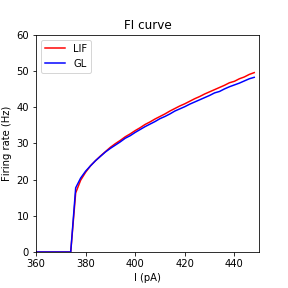
\includegraphics[width=\linewidth]{figures/FI_curve}
    \captionsetup{width=\linewidth}
    \captionof{figure}{FI curve of LIF (red) and GL (blue) neuron model.}
    \label{fig:FI_curve}
  \end{center}
  \begin{center}
    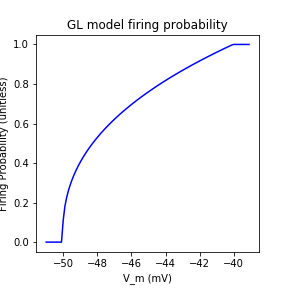
\includegraphics[width=\linewidth]{figures/GL_Phi}
    \captionsetup{width=\linewidth}
    \captionof{figure}{Firing rate ($\Phi(V)$) of the GL model.}
    \label{fig:GL_Phi}
  \end{center}
\end{multicols}

\paragraph{Implementation in python}

For the python implementation try to stick at most to numpy packages, and try to avoid packages as scipy and others. On the code bellow, np stands for numpy as the numpy module is loaded as follow. We also specify the seed for the random number generator: 

\textbf{Remark 1} Poissonian external input is not implemented yet on this version. The code will be updated accordingly, and reported when done.

\begin{minted}[bgcolor=shadecolor,fontsize=\scriptsize]{python}
import numpy as np
# random number generator depends on numpy version
# Here I used numpy 1.19:
self.rng = np.random.default_rng(seed=1234)
self.poisson_rng = np.random.default_rng(seed=2345)
# create an empty list to store spike activity
spk_neuron = []
spk_time = []
\end{minted}

\begin{enumerate}
    \item Creates an array containing $N$ neurons. The number of neurons is the sum of number of neurons per layer in table \ref{table:PD_num_neurons}:
\begin{minted}[bgcolor=shadecolor,fontsize=\scriptsize]{python}
V_m = np.zeros(N)
\end{minted}
    \item parameters $\rho$, $\xi$ and $\zeta$ are calculated using neuron parameters described above:
\begin{minted}[bgcolor=shadecolor,fontsize=\scriptsize]{python}
rho = np.exp(-dt/tau_m)
xi = np.exp(-dt/tau_syn)
zeta = ( np.exp(-dt/tau_m) - np.exp(-dt/tau_syn_ex) ) / ( 1/tau_syn - 1/tau_m )*C_m
\end{minted}
Store connectivity data as python dictionary (dictionary is an efficient way of accessing data):
\begin{minted}[bgcolor=shadecolor,fontsize=\scriptsize]{python}
conn_dict = {pre_id:{'target':[array of target neuron id],
                    'weight':[array of synaptic weights],
                    'delay':[array os synaptic delays]}
\end{minted}
    \item evolve time ($t$) and $V_t(i)$ are evaluated as:
\begin{minted}[bgcolor=shadecolor,fontsize=\scriptsize]{python}
t = 0.0
dt = 0.1
while t<= t_sim:
    t = t + dt
    V_m = rho*V_m + zeta*I_syn
\end{minted}
where summed\_weights is a 2D array containing the sum of synaptic inputs arriving at the neuron. the first index represents synaptic delays in step counts. Therefore, index 0 represents the effective synaptic inputs, that is, spikes that occurred d steps in the past, with d representing the delay. This 2D array is than shifted along the delay axes to accommodate the next \textit{effective} spike inputs.
{\color{blue}
    \item Draw Poissonian spike inputs
    \begin{minted}[bgcolor=shadecolor,fontsize=\scriptsize]{python}
    # generate poisson spike train for time window dt
    # convert time from ms to s (poisson_rate is in Hz, while dt is in ms)
    lambda_ = poisson_rate * dt * 1e-3
    poisson = poisson_rng.poisson(lambda_, N) # draw sample from a poisson distribution
\end{minted}
}
    \item evolve $I_syn(i)$ as:
\begin{minted}[bgcolor=shadecolor,fontsize=\scriptsize]{python}
    I_syn = xi * I_syn_ex + summed_weights[0] + poisson*weight
\end{minted}
where summed\_weights is a 2D array containing the sum of synaptic inputs arriving at the neuron. the first index represents synaptic delays in step counts. Therefore, index 0 represents the effective synaptic inputs, that is, spikes that occurred d steps in the past, with d representing the delay. This 2D array is than shifted along the delay axes to accommodate the next \textit{effective} spike inputs.
    \item Find for neurons in refractory period and reset its membrane potential and I\_syn
\begin{minted}[bgcolor=shadecolor,fontsize=\scriptsize]{python}
    idx_ref = np.where(is_ref > 0)[0]
    V_m[idx_ref] = V_reset
    I_syn_ex[idx_ref] = 0.0
    I_syn_in[idx_ref] = 0.0
\end{minted}
is\_ref is a counter that stores the number of simulation step necessary for the refractory period. Each time step this counter is decreased by one, therefore, when this counter is $\leq$ 0, indicates that the neuron is no more in its refractory period.
    \item calculate the firing probability function ($\phi(V)$):
\begin{minted}[bgcolor=shadecolor,fontsize=\scriptsize]{python}
    V_diff = V_m - V_rheo
    idx_neg = np.where(V_diff < 0)
    V_diff[idx_neg] = 0.0
    phi = np.power(gamma*V_diff, r)
\end{minted}
where V\_rheo is the rheobase potential, the minimum potential necessary for a neuron to spike, gamma=0.1 and r=0.4. V\_diff is clipped at zero to force all potentials below V\_rheo to have a firing probability of zero.
    \item draw an array of uniform random numbers, with array size equal to neuron population size, and choose which neuron has spiked.
\begin{minted}[bgcolor=shadecolor,fontsize=\scriptsize]{python}
    # if using python > 1.17:
    # U_i = self.rng_.random(self.N) # needs numpy > 1.17
    # I use numpy 1.16.2:
    U_i = np.random.uniform(size=self.N)
    # get index of neurons that spiked
    idx_spiked = np.where(phi >= U_i)[0]
\end{minted}
    \item set refractory count of the neurons that spiked
\begin{minted}[bgcolor=shadecolor,fontsize=\scriptsize]{python}
    is_ref[idx_spiked] = refractory_count
\end{minted}
    \item send spike event to postsynaptic neurons.synaptic weight is then sent to the target neuron as follow (spike activity is also stored to a variable and/or file):
\begin{minted}[bgcolor=shadecolor,fontsize=\scriptsize]{python}
    for pre in idx_spiked:
        for idx, post in enumerate(conn_dict[pre+1]['target']):
            idx_delay = int(conn_dict[pre+1]['delay'][idx]/dt) # delay step counts
            summed_weights[idx_delay][post-1] += conn_dict[pre+1]['weight'][idx]
        spk_neuron.append(pre+1)
        spk_times.append(t)
\end{minted}
\textbf{Remark 1} note that idx\_spike starts at zero, whereas neuron\_id starts at 1.

\textbf{Remark 2} If delays are all the same between pairs of neurons, the inner loop may be eliminated as:
\begin{minted}[bgcolor=shadecolor,fontsize=\scriptsize]{python}
    for pre in idx_spiked:
        summed_weights[idx_delay][conn_dict[pre+1]['target']-1] += conn_dict[pre+1]['weight']
        spk_neuron.append(pre+1)
        spk_times.append(t)
\end{minted}
    \item shift summed\_weight array discarding the transmitted weights, and adding zeros to the end of the array
\begin{minted}[bgcolor=shadecolor,fontsize=\scriptsize]{python}
    for idx in range(1,len(summed_weights)):
        summed_weights[idx-1] = summed_weights[idx]
    summed_weights[-1][:] = 0.0
\end{minted}
\textbf{Remark 3} Steps 3 -- 9 are within the same loop, and closes one simulation step.
\end{enumerate}

\color{black}
\color{blue}
\paragraph{Implementation in C++ -- Nilton}

ToDo: describe de C++ code by Nilton

\paragraph{Implementation in C -- Stolfi}

ToDo: Describe de C code by Stolfi
\color{black}

\subsection{Analysis of the GL model}
\label{sec:org1f80ff6}

\subsubsection{The firing probability curve revisited -- comparison with Stolfi's code}
\label{sec:org8017ec1}

\color{red}
ToDo: describe Stolfi's code somewhere.

Stolfi's code uses simulation time step (dt) of 1 ms. Fig. \ref{fig:DC_FI_9000} shows the FI-curve of the implemented GL neuron (C++ version) to a constant current input ranging from 300 -- 9000 pA varied in 100 pA steps, simulated for 10 seconds. Blue dots represents the FI-curve obtained by a dt of 0.1 ms, and orange dots by a dt of 1 ms.

Note that at dt of 1 ms, the firing rate saturates at about 333 Hz. This is due to the fact that the neuron has a refractory period (\(\tau_{ref}\)) of 2 ms. In such case, when a neuron fires at time \(t\), it will remain silent until time \(t+\tau_{ref}\), and the closes next spike will be at time \(t+\tau_{ref}+1\), resulting in a period of 3 ms which is about 333 Hz. This result 

On the other hand, at dt of 0.1 ms, the FI curve should saturate at nearly 500 Hz, as the shortest period will be 2.1 ms.

\begin{figure}
    \centering
    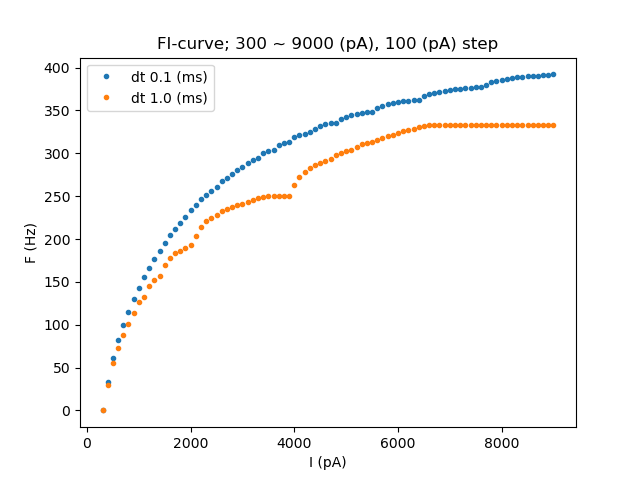
\includegraphics[width=0.6\linewidth]{figures/DC_FI_9000.png}
    \caption{FI-curve}
    \label{fig:DC_FI_9000}
\end{figure}

\subsubsection{Firing rate of a single neuron the the layer specific input}
\label{sec:orgf57c0d1}

The GL neuron was submitted to the layer specific external input shown in section \ref{sec:PD_original}.

\begin{table}[h]
    \centering
    \caption{Firing rate to layer specific constant input}
    \label{tab:DC_input_firing_rate}
    \begin{tabular}{l|rrr}
        \multicolumn{2}{c}{}& \multicolumn{2}{c}{firing rate (Hz)} \\
        layer & DC (pA) & dt=0.1 & dt=1 \\
        \hline
        L23E & 561.92 & 74.4 & 65.4 \\
        L23I & 526.8 & 67.0 & 60.1 \\
        L4E & 737.52 & 105.7 & 91.6 \\
        L4I & 667.28 & 94.1 & 82.2 \\
        L5E & 702.4 & 100.1 & 88.9 \\
        L5I & 667.28 & 94.2 & 82.8 \\
        L6E & 1018.48 & 145.4 & 127.4 \\
        L6I & 737.52 & 105.6 & 91.6
    \end{tabular}
\end{table}

\begin{table}[h]
    \centering
    \caption{Firing rate to layer specific constant input -- Stolfi version (dt=1(ms))}
    \label{tab:DC_input_firing_rate_Stolfi}
    \begin{tabular}{l|rrr}
        layer & $I_{avg}$ & $I_{dev}$ & firing rate (Hz) \\
        \hline
        L23E & 2.221 & 0.637 & 79.84 \\
        L23I & 2.115 & 0.627 & 69.86 \\
        L4E & 2.943 & 0.717 & 119.76 \\
        L4I & 2.678 & 0.638 & 109.78 \\
        L5E & 2.813 & 0.724 & 109.78 \\
        L5I & 2.636 & 0.686 & 99.80 \\
        L6E & 4.063 & 0.858 & 177.64 \\
        L6I & 2.990 & 0.711 & 121.76
    \end{tabular}
\end{table}

\color{black}

\subsection{Analysis of the PD model}
\label{sec:orgedd205f}

\subsubsection{Outdegree}
\label{sec:orgc683567}

Outdegree is the number of outgoing synapses. Fig. \ref{fig:PD_outdegree} shows the histogram of outdegrees in a realization of the PD model (NEST config: master$\backslash$\_seed=55; number of virtual processes=16)

\begin{figure}[h]
    \centering
    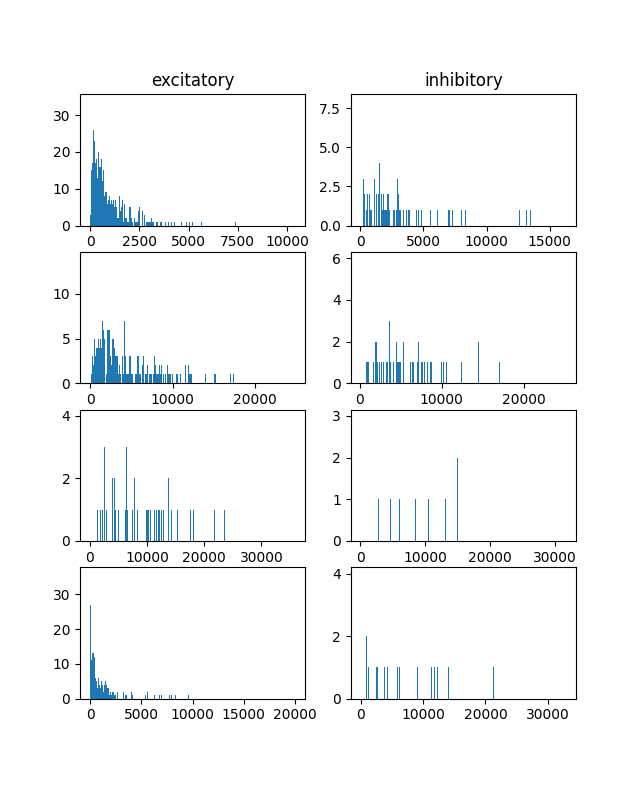
\includegraphics{figures/fig_outdegree.png}
    \caption{Caption}
    \label{fig:PD_outdegree}
\end{figure}

An example of maximum and minimum connection is shown in table \ref{table:PD_outdegree}.

\begin{table}[h]
    \centering
    \caption{Maximum and minimum outdegrees per layer}
    \label{table:PD_outdegree}
    \begin{tabular}{c||c|c}
         & max & min  \\
         L23e & 10414 & 4 \\
         L23i & 16270 & 51 \\
         L4e & 24829 & 19 \\
         L4i & 25087 & 127 \\
         L5e & 35869 & 67 \\
         L5i & 31656 & 72 \\
         L6e & 20025 & 0 \\
         L6i & 32872 & 19
    \end{tabular}
\end{table}

\section{Pseudo Random Number Generator (PRNG)}
\label{sec:org78260f4}

The pseudo random number generation is going to be done with the \href{https://en.wikipedia.org/wiki/Xoroshiro128\%2B}{Xoroshiro128+} algorithm using a \href{https://gist.github.com/siebenschlaefer/bfe750df9b7104ba4eed874223b8ab1f}{C++ wrapper implemented by Matthias Rahlf} of the \href{http://vigna.di.unimi.it/xorshift/xoroshiro128plus.c}{original C implementation} of \href{https://arxiv.org/abs/1805.01407}{Blackman and Vigna}. 
To obtain the different distributions (\emph{i.e.} real uniform [0, 1), ingeter uniform [min, max), normal distribution (\(\mu=0\), \$\(\sigma\)=1) and poisson distribution (\(\lambda\))), the standard library will be used.

\subsection{A test case of the PRNG}
\label{sec:org708cd29}

Here the generation of \(8\times 10^8\) uniformly distributed real numbers in the range [0, 1) will be drawn, and the time of execution measured for the cases of xoroshiro128+ and mt19937 (Mersenne Twister) generators, where the latter is present in the standard libray. the number of random number generated is approximatly the number of random numbers that will be necessary for simulating the PD microcircuit model for \(10^4\) steps.

\subsubsection{The xoroshiro128+ case}
\label{sec:org9dc6d38}

The code for drawing \(8\times 10^8\) uniformly distriburted random number with the xoroshiro128+ generator:

\begin{minted}[bgcolor=shadecolor,fontsize=\scriptsize]{c++}
#include "xoroshiro128plus.hpp"
#include <random>

xoroshiro128plus prng;
std::uniform_real_distribution<> udist;

int N=800000000;

int main() {
  double val;

  // seed half the maximal value
  prng.seed(prng.max()*0.5);

  for (int i=0; i<N; i++) {
    val = udist(prng);
  }
}
\end{minted}

Compiling the source code and measuring the execution time:

\begin{minted}[bgcolor=shadecolor,fontsize=\scriptsize]{sh}
g++ ./src/test_prng_xoroshiro128plus.cpp -o ./src/run_test_prng_xoroshiro128plus
time ./src/run_test_prng_xoroshiro128plus
\end{minted}

\begin{verbatim}

real	0m25.935s
user	0m25.911s
sys	0m0.000s
\end{verbatim}


\subsubsection{The mt19937 case}
\label{sec:org4f6ce2d}

The code for drawing \(8\times 10^8\) uniformly distriburted random number with the mt19937 generator:

\begin{minted}[bgcolor=shadecolor,fontsize=\scriptsize]{c++}
#include <random>

std::mt19937 prng;
std::uniform_real_distribution<> udist;

int N=800000000;

int main() {
  double val;

  // seed half the maximal value
  prng.seed(prng.max()*0.5);

  for (int i=0; i<N; i++) {
    val = udist(prng);
  }
}
\end{minted}

Compiling the source code and measuring the execution time:

\begin{minted}[bgcolor=shadecolor,fontsize=\scriptsize]{sh}
g++ ./src/test_prng_mt19937.cpp -o ./src/run_test_prng_mt19937
time ./src/run_test_prng_mt19937
\end{minted}

\begin{verbatim}

real	0m0.060s
user	0m0.058s
sys	0m0.001s
\end{verbatim}

\subsubsection{Which is faster?}
\label{sec:orgf4dba14}

For a very simple code that just generates uniformly distributed random numbers, the xoroshiro128+ algorithm was about 33\% faster than the widely used mt19937 generator.




\end{document}
\end{document}
